\documentclass[tikz,border=14pt]{standalone}
\usetikzlibrary{arrows.meta}
\begin{document}
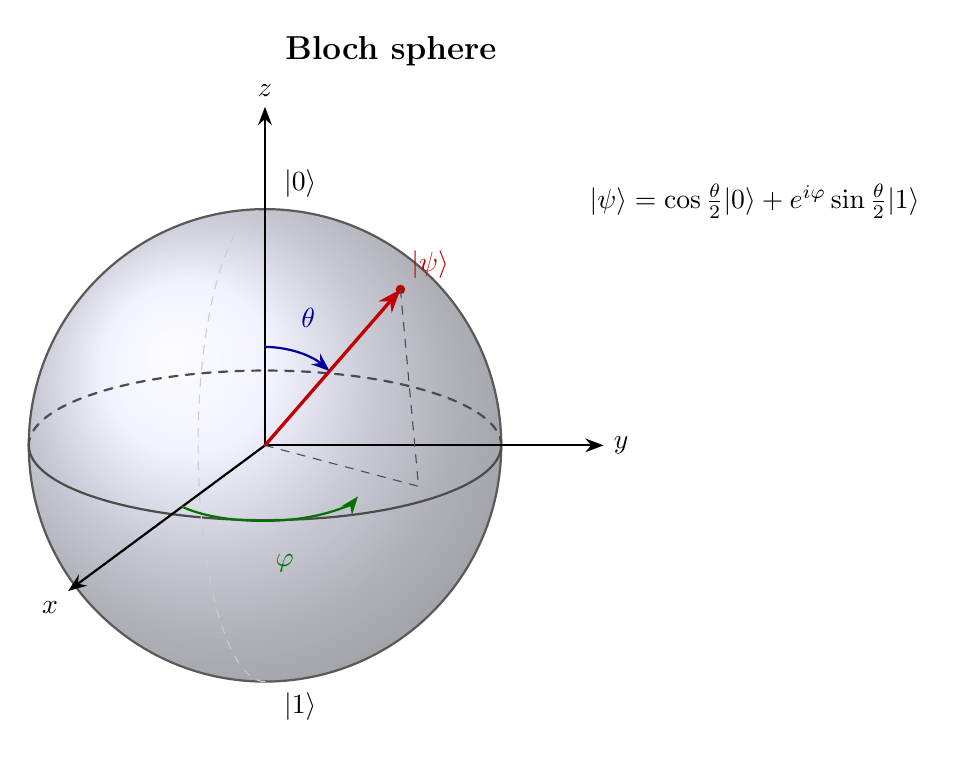
\begin{tikzpicture}[>=Stealth,line cap=round,line join=round,font=\normalsize]

  \def\R{3}

  % sphere body
  \shade[ball color=blue!12,opacity=0.55] (0,0) circle (\R);
  \draw[gray!70!black,thick] (0,0) circle (\R);

  % equator (dashed back half, solid front half)
  \draw[gray!60!black,thick] (-\R,0) arc[start angle=180,end angle=360,
    x radius=\R,y radius=0.95];
  \draw[gray!60!black,thick,dashed] (\R,0) arc[start angle=0,end angle=180,
    x radius=\R,y radius=0.95];

  % meridian for depth
  \draw[gray!40,dashed] (0,-\R) arc[start angle=270,end angle=90,
    x radius=0.85,y radius=\R];

  % axes
  \draw[->,thick] (0,0) -- (0,4.3) node[above] {$z$};
  \draw[->,thick] (0,0) -- (-2.5,-1.85) node[below left] {$x$};
  \draw[->,thick] (0,0) -- (4.3,0) node[right] {$y$};

  % basis state labels
  \node[anchor=south west] at (0.12,3.02) {$|0\rangle$};
  \node[anchor=north west] at (0.12,-3.02) {$|1\rangle$};

  % state vector |psi>
  \coordinate (P) at (1.72,1.98);
  \draw[->,very thick,red!75!black] (0,0) -- (P)
    node[above right] {$|\psi\rangle$};
  \fill[red!75!black] (P) circle (0.06);

  % projection onto equatorial plane
  \coordinate (Q) at (1.95,-0.52);
  \draw[gray!60!black,dashed] (P) -- (Q);
  \draw[gray!60!black,dashed] (0,0) -- (Q);

  % theta arc (from z axis to state vector)
  \draw[->,thick,blue!60!black] (0,1.25) arc[start angle=90,end angle=49,radius=1.25];
  \node[blue!60!black] at (0.55,1.62) {$\theta$};

  % phi arc (from x axis to projection, along equator)
  \draw[->,thick,green!45!black] (-1.05,-0.78) arc[start angle=215,end angle=345,
    x radius=1.25,y radius=0.42];
  \node[green!45!black] at (0.25,-1.5) {$\varphi$};

  % state formula
  \node[align=center,anchor=west] at (4.0,3.1)
    {$|\psi\rangle=\cos\frac{\theta}{2}|0\rangle+e^{i\varphi}\sin\frac{\theta}{2}|1\rangle$};

  % title
  \node[font=\bfseries\large] at (1.6,5.0) {Bloch sphere};
\end{tikzpicture}
\end{document}
